\chapter{Partially Observable Markov Decision Processes}

Until now we have considered the case of fully observable \glspl{mdp}, 
where the agent has access to the complete state of the environment. However, this is not always the case, 
and in many real-world scenarios, the agent has only partial information about its surroundings. 
As \glspl{mdp} are controlled Markov Chains, \glspl{pomdp} are controlled Hidden Markov Models. \Cref{fig:pomdp}
shows how the underlying process states are hidden from the agent, which can only observe the environment 
through its sensors.
\begin{figure}[H]
    \centering
    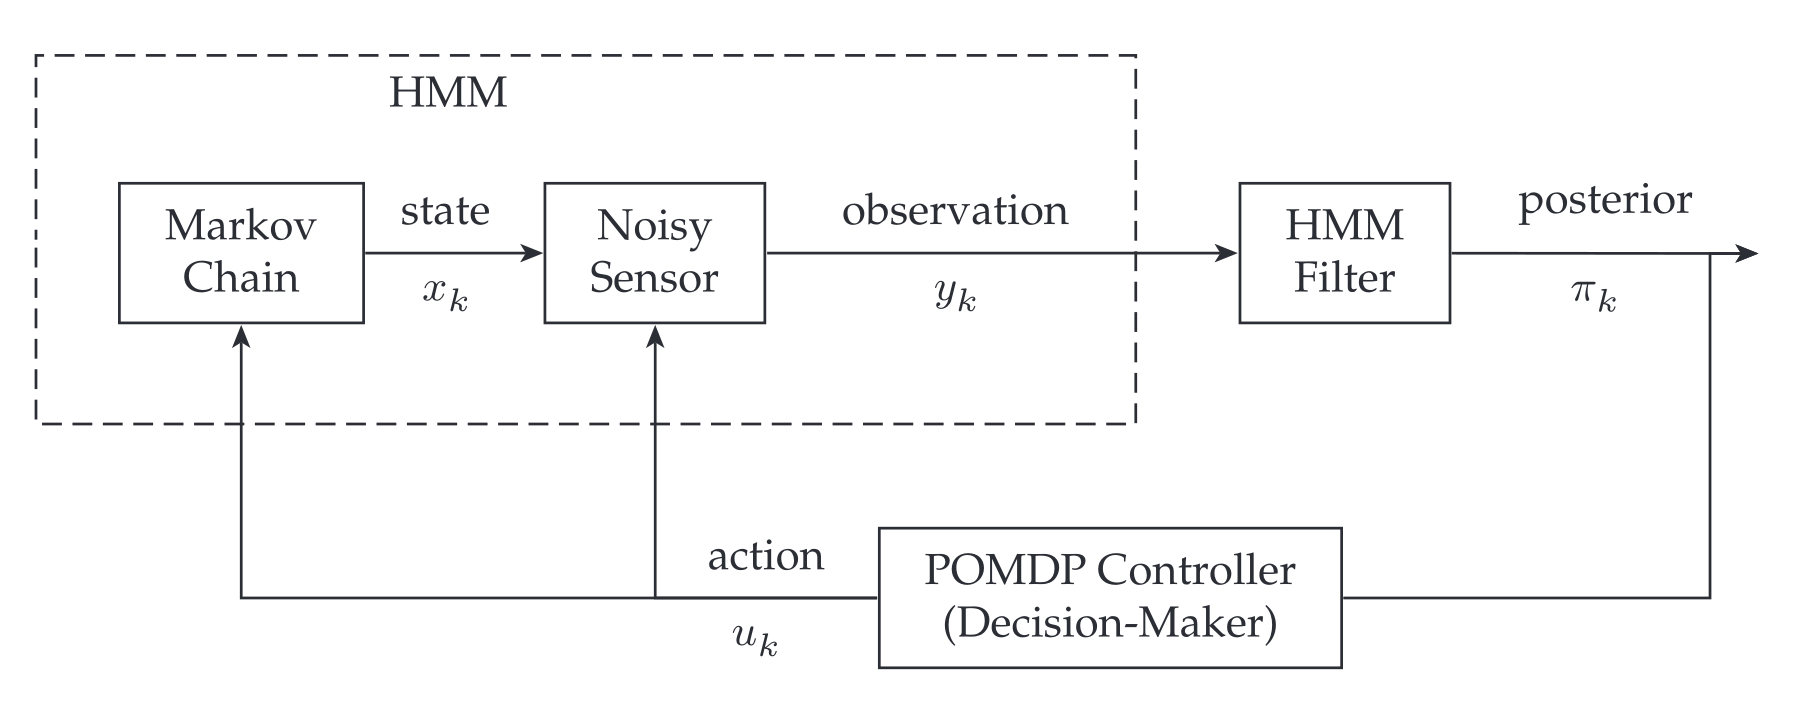
\includegraphics[scale=.15]{images/pomdp.png}
    \caption[Partially Observable Markov Decision Process]{Partially Observable Markov Decision Process \citep{Krishnamurthy_2016}}
    \label{fig:pomdp}
\end{figure}
As such, \glspl{pomdp} are an extension of \glspl{mdp} to the case where the full observability assumption is 
relaxed in favour of a more general and realistic assumption that the agent only has partial knowledge 
of the state of the system but there exist observations/signals which yield probabilistic beliefs about 
the hidden state.

The next sections will be based on \cite{Spaan12pomdp} and \cite{Hauskrecht_2000} analysis of \glspl{pomdp},
originally introduced by the work of \cite{drake1962observation} \cite{1307539f-051d-3d3c-a0d8-111443bed03f},
\cite{ASTROM1965174} and \cite{10.1007/BF02055574}.


\begin{definition}
A \textit{Partially Observable Markov Decision Process} is a tuple $P = (S, A,\Omega, \mathcal{T}, \mathcal{R}, \mathcal{O})$ where:
\begin{itemize}
    \setlength\itemsep{0.01em}
    \item $S$ is a finite set of states
    \item $A$ is a finite set of actions
    \item $\Omega$ is a finite set of observations
    \item $\mathcal{T}$ is the transition function $\mathcal{T} : S \times A \times S \rightarrow [0,1]$
    \item $\mathcal{R}$ is the reward function $\mathcal{R} : S \times A \times S \rightarrow \mathbb{R}$
    \item $\mathcal{O}$ is the observation function $\mathcal{O} : S \times A \times \Omega \rightarrow [0,1]$
\end{itemize}
\end{definition}

\begin{example}    
    Consider the two-state infinite-horizon \gls{pomdp} by \cite{NIPS1994_1c1d4df5} depicted in \ref{fig:memory}. The \gls{pomdp} is 
    defined by two states and two possible actions in each state. The agent receives an observation 
    independent of the state, and the reward is $r$ if the agent changes state and $-r$ otherwise.

    The optimal policy in the underlying \gls{mdp} is to take action $a^2$ in state $s^1$ and 
    action $a^1$ in state $s^2$, yielding a reward of $r$ in each time step and producing an 
    optimal value function $V^*(s)=\frac{r}{1-\gamma}$ by geometric series convergence. 
    
    In the \gls{pomdp}, the agent receives the same observation in both states, and 
    as a result, there are only two memoryless stationary deterministic policies possible: always taking action $a^1$ or always taking action $a^2$.
    Both policies yield a maximum expected reward of $r+\frac{\gamma r}{1-\gamma}$ if fortunate enough to take 
    the first action that leads to a different state. The best stationary stochastic policy would otherwise 
    be able to achieve an expected discounted reward of 0, when it chooses either action 50\% of the time, still 
    far from the optimal value of the \gls{mdp}.

    However, if the agent could remember what actions it had executed, it could execute a policy that 
    alternates between the two actions, achieving  $\frac{\gamma r}{1-\gamma}-r$ in the worst case.
\end{example}

\begin{figure}[H]
    \centering
    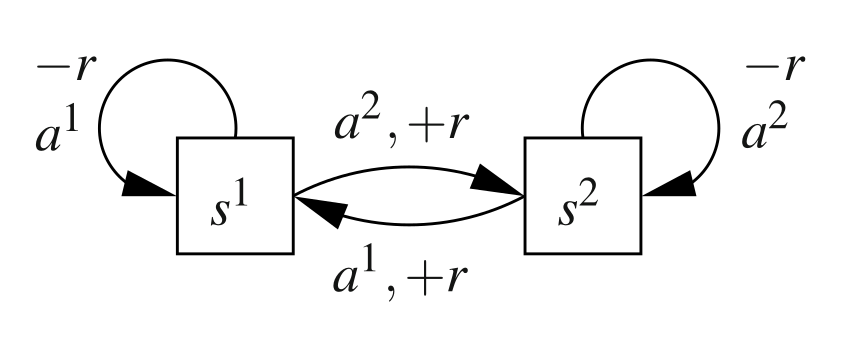
\includegraphics[scale=.2]{images/memorypomdp.png}
    \caption{The need for Memory}
    \label{fig:memory}
\end{figure}

This example shows how the lack of memory can severely limit the agent's ability to solve the problem.
In the next sections, we will introduce the main concepts and algorithms used to solve \gls{pomdp}s based on 
the formalization of the concept of memory.

\section{Belief State MDPs}
Since in \glspl{pomdp}, the underlying process states are unknown, the action choices will be based on the information available 
to the agent in the form of past actions and observations, giving rise to the concept of \textit{Information State}.

\begin{definition}
    (Complete Information State) The complete information state at time $t$, denoted
    $I_t$, consists of:
    \begin{itemize}
        \item[-] prior belief $b_0$ on states in $S$ at time $t=0$;
        \item[-] a complete history of actions and observations $\{o_0,a_0,o_1, ..., o_{t-1},a_{t-1},o_t\}$
    \end{itemize}
\end{definition}

A sequence of information states defines a controlled Markov process called 
information-state \gls{mdp}. In this context, a policy $\pi: I \rightarrow A$ is a mapping of 
information states to actions (possibly distributions over actions).
The new information state $I_{t+1}$ is obtained by applying an update function $\tau$ to the
the previous state $I_t$, previous action $a_{t-1}$ and observation $o_t$:
$$\tau: \mathcal{I} \times A \times O \rightarrow \mathcal{I}$$

It's easy to see that a \gls{pomdp} can be cast into the information-state MDP by using complete 
information states, revisiting the \gls{pomdp} such that states become information-states while transitions 
and rewards are updated according to:
$$\mathcal{R}(I,a) = \sum_{s s'} \mathcal{T}(s,a,s')\mathcal{R}(s,a,s')P(s|I) $$
$$\mathcal{T}(I,a,I') = \sum_o \tau(I,a,o)P(o|I,a) $$


It's also important to note that the information available can be also summarized in the 
so-called \textit{sufficient information states}. Such states must preserve
the necessary information content as well as the Markov property of the information-state.
\begin{definition}
    
    (Sufficient information state process). Let \(\mathcal{I}\) be an information state space 
    and \(\tau: \mathcal{I} \times A \times \Theta \rightarrow \mathcal{I}\) be an update function defining an information process \(I_{t}=\) 
    \(\tau\left(I_{t-1}, a_{t-1}, o_{t}\right)\). The process is sufficient with regard to the optimal control 
    if for every time step $t$, it satisfies:
    $$P\left(s_{t} \mid I_{t}\right)=P\left(s_{t} \mid I_{t}^{C}\right)$$
    $$P\left(o_{t} \mid I_{t-1}, a_{t-1}\right)=P\left(o_{t} \mid I_{t-1}^{C}, a_{t-1}\right)$$
    where \(I_{t}^{C}\) and \(I_{t-1}^{C}\) are complete information states.

\end{definition} 
% \todo{definisci meglio p(s|I) e p(o|I,a)?? è necessario?}

Being able to define a sufficient information state process is crucial since it allows us to avoid 
the curse of dimensionality of enlarging complete information states.

This brings us to the most common concept of \textit{belief state} as a form of sufficient information state
\cite{strm1965OptimalCO}.

A belief is a probability distribution over the states of the system which summarizes the history of 
actions and observations. Each \gls{pomdp} assumes an initial belief $b_0$, then at each time step
the belief is updated by the observation and the action taken through Bayes' rule:
\begin{equation}
    \tau(b,a,o) = b^{ao}(s')=\displaystyle\frac{p(o|s',a)}{p(o|b,a)}\sum_{s\in S}p(s'|s,a)b(s)
    \label{eq:beliefupdate}
\end{equation}

where $p(s'|s,a) = T(s,a,s')$ and $p(o|s',a) = O(s,a,o)$, and
$$p(o|b,a)=\displaystyle\sum_{s'\in S}p(o|s',a)\sum_{s\in S}p(s'|s,a)b(s)$$.

It is thus possible to define a \gls{mdp} over belief states. 
This transformation requires the transition and observation functions to be known
to the agent, and hence can be applied only in model-based methods.

The key point is that belief-state \glspl{mdp} are fully
observable even though the original problem involves hidden quantities. This
formulation effectively turns the problem into a planning one in the space of beliefs.

Belief-state MDPs are the primary object of study in the field of \glspl{pomdp}.

\section{Policies and Value Functions}
As in the fully observable context, the goal of the agent is to find a policy that maximizes the expected 
return. In the \gls{pomdp} case, the policy is a mapping from the set of probability distributions 
over $S$ to a probability distribution over actions $\pi : \Delta(S) \rightarrow \Delta(A)$ 
and the value function $V^{\pi} : \Delta(S) \rightarrow \mathbb{R}$. 
In the infinite-horizon discounted case, the value function is defined as:

$$V^{\pi}(b) \doteq \mathbb{E}_{\pi}\left[ \sum ^\infty _{t=0} \gamma^k \mathcal{R}(b_t,\pi(b_t)) | b_0 = b  \right]$$

where $\mathcal{R}(b_t,\pi(b_t)) = \sum_s \mathcal{R}(s,\pi(b_t))b_t(s)$.


Revisiting equations in the previous section, the Bellman optimality equation for the value function 
in a belief space \gls{mdp} is given by:
$$V^* (b) = \max_a \left[\sum_s R(s,a)b_t(s) + \gamma\sum_o p(o|b,a) V^*(b'_{a,o}) \right]$$

or alternatively, $V^* = HV^*$ where $H$ is the Bellman backup operator for \gls{pomdp}s defined as:
$$H V(b) = \max_a \left[\sum_s \mathcal{R}(s,a)b(s) + \gamma\sum_o p(o|b,a) V(b'_{a,o}) \right]$$

The properties of the H operator are sufficient to guarantee the existence of a unique optimal value 
function given the Banach contraction theorem. \textit{Exact Value Iteration} is therefore formulated 
as the iterative application of the H operator to an initial value function until convergence - practically 
until the difference between the value function at two consecutive iterations is below a given threshold.
\todo{serve una dimostrazione H contrazione}
$$V^{n+1} = HV_n = H^n V_0$$ 


The major difficulty in applying exact value iteration is that the belief space is continuous, and 
updates over the whole space are infeasible. 
Fortunately, the value function can be parameterized by a finite set of vectors; the following result 
is originally from \cite{1307539f-051d-3d3c-a0d8-111443bed03f}.

\begin{theorem}
    (Piecewise linear and convex Value function). Let \(V_{0}\) be an initial value function
    that is piecewise linear and convex. Then the \(i\)-th value function obtained after a finite
    number of update steps for a belief-state \gls{mdp} is also finite, piecewise linear and convex,
    and is equal to:
   
   \[
   V_{i}(b)=\max _{\alpha_{i} \in \Gamma_{i}} \sum_{s \in S} b(s) \alpha_{i}(s)
   \]
    where \(b\) and \(\alpha_{i}\) are vectors of size \(|S|\) and \(\Gamma_{i}\) is a finite set of vectors (linear functions) \(\alpha_{i}\).
\end{theorem}
\begin{proof}
It follows from induction. The result holds for the horizon one value function
$V_0 = \sum_s \mathcal{R}(s,a)b(s)= \sum_{i}b_i\alpha_{0}^{i}(s)= b \cdot \alpha_0 $
Assuming the hypothesis holds for \(V_n\), we can show that it holds for \(V_{n+1}\) as well.
\begin{align*}
    V_{n+1}(b)&=\displaystyle\max_{a}\Big[\sum_s \mathcal{R}(S,a)b(s)+\gamma\sum_{o}p(o|a,b)V_{n}(b_{a}^{o})\Big] \nonumber\\
    &=\displaystyle\max_{a}\Big[b\cdot r_{a}+\gamma\sum_{o}p(o|a,b)\max_{\{\alpha_{n}^{i}\}_{i}}\sum_{s^{\prime}}b_{a}^{o}(s^{\prime})\alpha_{n}^{i}(s^{\prime})\Big] \nonumber\\
    &=\displaystyle\max_{a}\Big[b\cdot r_{a}+\gamma\sum_{o}\max_{\{\alpha_{n}^{i}\}_{i}}\sum_{s^{\prime}}p(o|s^{\prime},a)\sum_{s}p(s^{\prime}|s,a)b(s)\alpha_{n}^{i}(s^{\prime})\Big] \nonumber\\
    &=\displaystyle\max_{a}\Big[b\cdot r_{a}+\gamma\sum_{o}\max_{\{g_{a,o}^{i}\}_{i}}b\cdot g_{a,o}^{i}\Big], \nonumber\\
    &=\displaystyle\max_{a}\Big[b\cdot r_{a}+\gamma b \cdot \sum_o arg\max_{\{g_{a,o}^{i}\}_{i}}b\cdot g_{a,o}^{i}\Big], \nonumber\\
    &=\displaystyle\max_{g_{a}^b}b \cdot g_a^b \nonumber
\end{align*}
denoting 
\[
\quad g_{a,o}^{i}(s)=\sum_{s^{\prime }}p(o|s^{\prime },a)p(s^{\prime
}|s,a)\alpha _{n}^{i}(s^{\prime }).\quad  
\]
and 
$$g_a^b = r_{a}+\gamma \sum_o arg\max_{\{g_{a,o}^{i}\}_{i}}b\cdot g_{a,o}^{i} $$

therefore one can express the value function as stated.

\end{proof}

\begin{remark}
    Even though the optimal value function for an infinite-horizon
    \gls{pomdp} is convex, it may not be piecewise linear. Nonetheless, it can be approximated
    arbitrarily closely by a piecewise linear and convex value function.
\end{remark}


The main idea behind most value iteration algorithms is that for a given value function 
\(V_{n}\) and a single belief point \(b\), we can
easily compute the vector \(\alpha_{n+1}^{b}\) of \(H V_{n}\) such that:
$$\alpha_{n+1}^{b}=\arg \max _{\left\{\alpha_{n+1}^{i}\right\}_{i}} b \cdot \alpha_{n+1}^{i}$$    
where \(\left\{\alpha_{n+1}^{i}\right\}_{i=1}^{|H V_{n}|}\) is the (unknown) set of vectors for \(H V_{n}\). 
We will denote this operation
\(\alpha_{n+1}^{b}=\operatorname{backup}(b)\). 
It computes the optimal vector for a given belief \(b\) by back-projecting:
\begin{equation}
    {backup}(b)=\arg\max_{g_a^b} b\cdot g_a^b
    \label{eq:backup}
\end{equation}
        
% \todo{copiato da perseus dal teorema a qui}

Due to the convexity of the value function, the expected discounted reward typically increases 
as the entropy of b decreases \Cref{fig:pomdp-value}. This remark is the basis for 
many entropy-regularized algorithms in \gls{pomdp}s.

\begin{figure}
    \centering
    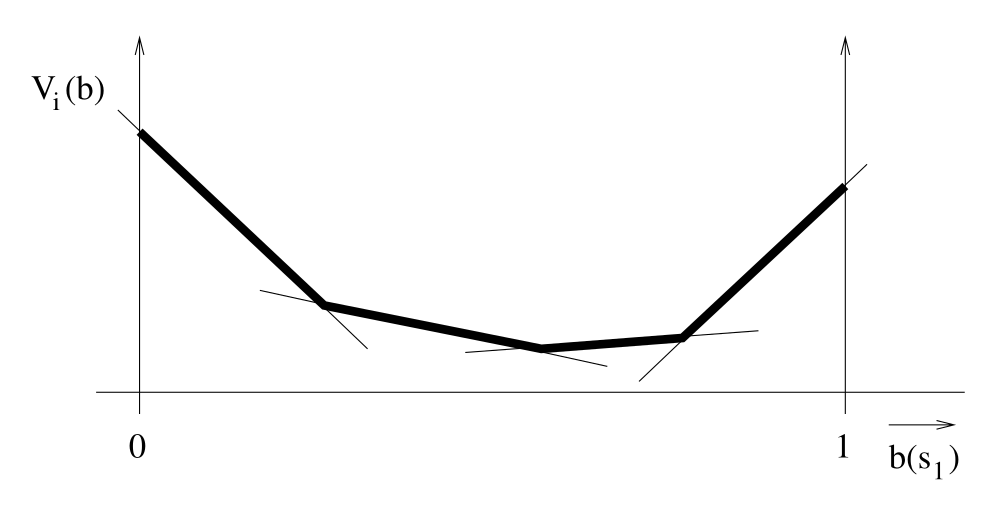
\includegraphics[scale=0.2]{images/pomdp-value.png}
    \caption{Convex Value function for a two states \gls{pomdp}.}
    \label{fig:pomdp-value}
\end{figure}


The total number of all its possible linear functions is $|A|\Gamma_i|^{|O|}$ (one
for every combination of actions and permutations of $\alpha_i$ vectors of size $|O|$). 
% per trovare il massmo dentro le [] devo fissare azione e per ogni osservazione trovare l'alpha vector
% precedente associato che massimizza le somme su ss'

\paragraph{Policy}
Similarly to the \gls{mdp} case, in \glspl{pomdp}, the optimal policy with respect to the Value function $V$ is:
$$\pi_{V}(b)=\underset{a}{\operatorname{argmax}} \left[\mathcal{R}(b, a)+\gamma \sum_{o \in \Omega} P\left(o \mid b, a\right) V\left(b^{a, o}\right)\right]$$

Computing a policy for the current belief state \(b\) using the above equation requires computing
all the \(|A| \times|\Omega|\) successors of \(b\), with a cost of \(|S|^{2}\) for each successor. 
Then, computing the value at each successor requires \(|S| \times|\Gamma|\) operations 
(using the \(\alpha\)-vector representation).

However, we can label the vector resulting from the
point-based backup operation with the action associated with it. 
Then, all we need is to find the best $\alpha$-vector for the current
belief state and execute the corresponding action, with a computation cost of only $|S|\times|\Gamma|$ for 
finding the best action when following V.

\section{Exact Value Iteration}
The process of \emph{exact value iteration} \cite{c6635fb4-4e99-3bcb-ba95-fb8ac7476062} \cite{doi:10.1287/mnsc.28.1.1},
starts by enumerating all possible linear functions:
\[
    H_{POMDP}V_{n}=\bigcup_{a}\;G_{a},\;\;\mathrm{with}\;\;G_{a}=\bigoplus_{o}\Big\{\frac{1}{%
    |\Omega|}r_{a}+\gamma g_{a,o}^{i}\Big\}_{i}  
\]
Since the complete set of linear functions is rarely needed (some of the linear functions are 
dominated by others, therefore not affecting the value function), redundant vectors are then pruned:
$$V_{n+1} = prune(H_{POMDP}V_n)$$

Incremental pruning strategies by \cite{10.5555/2074226.2074233} can be adopted to reduce the computational 
cost of the pruning linear program. Still, the pruning steps are usually expensive and seem to make a difference
only in the constant factors rather than the order of growth of needed vectors.
    
In each iteration, the value function is updated across the entire belief space, vectors $G_a$ 
are $|\Gamma| \times |A| \times |\Omega|$ and each one is computed in $|S|^2$ operations. Then, we 
create \(|\Gamma|^{\Omega|}\) new vectors for each action, with a complexity of \(|S|\) for each new 
vector. The overall complexity of a single iteration is \(O\left(|\Gamma| \times|A| \times|\Omega| \times|S|^{2}+|A| \times|S| \times|\Gamma|^{\Omega|}\right)\).

% Recent extensions of the
% method interleave the generate and test stages and do early pruning on a set of partially
% constructed linear functions (Zhang  Liu, 1997a; Cassandra, Littman,  Zhang, 1997;
% Zhang  Lee, 1998).
An alternative to this approach relies on the idea of computing a useful linear function for a
single belief state, and then defining a set of constraints over the belief space where this vector 
is guaranteed to be dominant (Sondik, 1971; Smallwood  Sondik, 1973).

The main challenge is identifying all belief points that seed valuable linear functions. 
Approaches to address this include Sondik's one- and two-pass algorithms \cite{c6635fb4-4e99-3bcb-ba95-fb8ac7476062}, 
Cheng's methods \cite{Cheng_1988}, and the Witness algorithm 
\cite{10.5555/864404,10.5555/2891730.2891888}.

\section{Point Based Value Iteration}
Approximate solution methods are necessary to solve \glspl{pomdp} in practice, since even modest 
sized problems are intractable with exact methods.
The main assumption behind \gls{pbvi} by \cite{10.5555/1630659.1630806} is that
it is unlikely to reach most of the points in the belief simplex.
Computing solutions only for those parts of the belief simplex that are reachable, i.e.,
that can be actually encountered by interacting with the environment, can drastically reduce 
the computational complexity of the problem.

The \gls{pbvi} algorithm solves a POMDP for a finite set of belief points $B$
initializing an $\alpha$-vector for each $b \in B$, and repeatedly updating 
(via value backups) the value of that $\alpha$-vector, preserving the piecewise linearity 
and convexity of the value function, and defining a value
function over the entire belief simplex.
\begin{figure}[H]
    \centering
    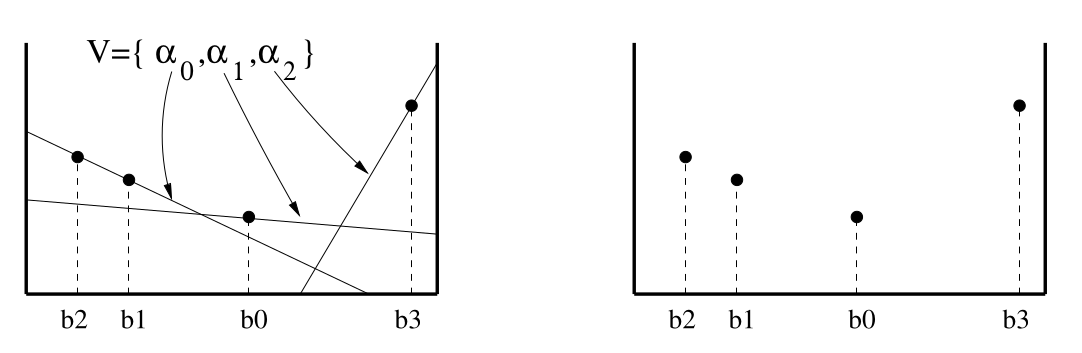
\includegraphics[scale=.35]{images/pbvi.png}
    \caption{Point-Based Value Iteration}
    \label{fig:pbvi}
\end{figure}



The point-based update follows exactly Eq. \ref{eq:backup} for each belief point in the set $B$. 
This is repeated h times for finite h-horizon problems, or a predefined number of iterations in the 
infinite case.

The next step is to enlarge the set of belief points by selecting for each belief \(b\) in \(B\) 
a successor \(b^{\prime}\) that is the most distant from the set \(B\). That is, let \(L\) be a 
distance metric, then define:
\[
\left|b^{\prime}-B\right|_{L}=\min _{b \in B}\left|b-b^{\prime}\right|_{L}
\]

and focus on candidate successors generated using forward simulation, thus:

\[
b^{\prime}=\max _{a, o}\left|b^{a, o}-B\right|_{L}
\] 

The set of successor points, one b for each b in $B_{i-1}$ , are added into Bi (along with the previous
points in Bi ) to create the new set Bi+1 . Experiments by various researchers show little, if
any, sensitivity to the distance metric chosen, and L 1 has useful theoretical properties for the
convergence of PBVI. The full procedure is formally described in Algorithm


% The complexity of computing $g_{a,o}^{i}$ is \(O\left(|S|^{2}\right)\), and it is done for every \(\alpha \in V\), hence
%  computing all $g^{a, o}$ requires \(O\left(|A| \times|\Omega| \times|V| \times|S|^{2}\right)\). Computing \(\alpha_{a}^{b}\) (Eq. 34) requires the
%  computation of all the relevant \(\alpha^{a, o}\), but then the summation and inner products require only
%  \(O(|S| \times|\Omega|)\) operations and another \(O(|S|)\) operations for adding the reward vector. Finally,
%  the backup operation requires for each \(\alpha_{a}^{b}\) another \(O(|S|)\) operations for the inner
%  product. Hence, the full complexity of the point-based backup requires \(O(|A| \times|\Omega| \times|V| \times\)
%  \(|S|^{2}+|A| \times|S| \times|\Omega|\) ).

As per previous analysis, the complexity of the point-based backup on a single belief is 
\(O(|A| \times|\Omega| \times|V| \times|S|^{2}+|A| \times|S| \times|\Omega|\) ).
However, a full backup for the subset \(B\) will not require \(|B|\) times the complexity of a
single point-based backup, because the \(g^{a, o}\) are independent of the current belief point \(b\).
Hence, executing a backup for \(|B|\) belief points over a single value function \(V\), where we
compute every \(g^{a, o}\) only once, requires \(O(|A| \times|\Omega| \times|V| \times|S|^{2}+\)
\(|B| \times|A| \times|S| \times|\Omega|\) ), as compared with the \(O(|A| \times|\Omega| \times|V| \times|S|^{2}+|A| \times|S| \times|V|^{\Omega|})\)
of a single iteration of the exact backup. 

For any belief set $B$ and horizon $n$, \gls{pbvi} produces an estimate \(V_{n}^{B}\) such that the 
error between \(V_{n}^{B}\) and the true value function \(V^*_{n}\) is bounded, and the bound 
depends on how dense $B$ is in the Belief space \cite{10.5555/1630659.1630806}. \\

\gls{pbvi} represents a class of algorithms based on the above ideas. They differ mainly in 
in how new belief points are selected, in how belief points are updated in each
backup iteration, and in other minor optimizations, such as pruning techniques
or better initial value functions. 
In general, these algorithms always interleave belief point collection and belief point updates.

\subsection{Perseus}
Perseus by \cite{Spaan_2005} introduces a method to reduce the number of belief updates required at each iteration,
while still improving the value function for a large number of beliefs. With fewer belief point 
updates per step, there is room for many more iterations of belief point updates, for a given 
time constraint. 

% The Perseus algorithm is best described by the pseudocode in \cref{alg:perseus}. 

% \begin{algorithm}
%     \caption{Perseus: Point-Based Value Iteration for POMDPs}\label{alg:perseus}
%     \begin{algorithmic}
%     \Require A POMDP defined by $(S, A, Z, T, O, R, \gamma)$, a set of sampled belief points $\mathcal{B}$, and number of iterations $N$
%     \Ensure Approximate value function $V$ and policy $\pi^*$
    
%     \State Initialize value function $V_0$ arbitrarily over belief space
%     \For{$n = 1$ to $N$}
%         \State $V_n \gets \emptyset$
%         \State Copy belief set: $\mathcal{B'} \gets \mathcal{B}$
%         \While{$\mathcal{B'} \neq \emptyset$}
%             \State Select a random belief $b \in \mathcal{B'}$
%             \State Compute backup: $\alpha_{b}^{a^*} \gets backup(b)$
%             \State Store corresponding alpha vector $\alpha_{b}^{a^*}$ in $V_n$
%             \State Remove all beliefs in $\mathcal{B'}$ for which $V_n$ improves upon $V_{n-1}$
%         \EndWhile
%     \EndFor
%     \State Extract policy: $\pi^*(b) \gets \arg\max_{a \in A} \sum_{s \in S} b(s) \alpha^a(s)$ for all $b \in \mathcal{B}$
%     \State \Return $V_N, \pi^*$
%     \end{algorithmic}
% \end{algorithm}

It starts with running random exploration in belief space, collecting belief points 
until a (relatively) large number of points are collected.

Then, given a previous value function $V_n$, the Perseus backup stage is performed: 
$$V_{n+1} = \tilde{H}_{Perseus} V_n$$ 
The operator is built such that $V_{n+1}$ improves the value of all $b \in B$:
upper bounds $V_n$ over $B$ (but not necessarily over $\Delta(S)$ which would require linear programming):
$$V_{n+1}(b) \geq V_n(b) \quad \forall b \in B$$

$\tilde{H}_{Perseus}$ defines a set $\tilde{B} = B$ and a new empty
value function $V_{n+1} = \emptyset$. A belief point $b \in \tilde{B}$ is then selected uniformly at random and used to
compute a new vector $\alpha_{new} = backup(b,V_n)$. If $\alpha_{new}\cdot b > V_n(b)$, then $\alpha_{new}$ is added into
$V_{n+1}$, and we remove from $\tilde{B}$ all $b'$ such that $\alpha_{new} \cdot b' > V_{n+1}(b')$. 
That is, all belief points whose value was improved by $\alpha_{new}$ will not be backed up at the 
current iteration. If $\alpha_{new} \cdot b \leq V_n (b)$, 
we add $\alpha_{old} = argmax \alpha \in V_n \alpha \cdot b$ into $V_{n+1}$. 
The iteration ends when $\tilde{B} = \emptyset$, and $V$ is set to $V'$.

Note however that in this algorithm, it is assumed that if $\alpha_{new} \cdot b > V_m(b)$,
then $|\alpha_{new} \cdot b - V^*(b)| < |V_n(b) - V^* (b)|$. 
This is only true if we initialize $V$ to a lower bound on $V^*$ . Therefore, unlike \gls{pbvi}, 
Perseus requires a lower bound initialization $V_0 = \set{\alpha_0}$ such that:
$$\alpha_0 = \frac{1}{1-\gamma}min_{s,a}\mathcal{R}(s,a)$$

The key advantages over \gls{pbvi} are that the belief collection step is fast, and the value function
update tends to be represented by a number of $\alpha$-vectors much smaller than $|B|$.
Thus, Perseus can collect a set of belief points much larger than \gls{pbvi}.

This comes at some cost; first, the random belief
gathering assumes that it is relatively simple to obtain good belief points, 
which also represents a practical limitation in domains that require long trajectories.
Second, even though the value for every point $b \in B$ gets closer to $V^*(b)$ with every
iteration, many belief points will not get backed up and the value function may remain far from
optimal for many beliefs. 

\section{MDP based Approximations}

To address challenges arising from the curse of dimensionality (the belief space is continuous and high-dimensional) 
and the curse of history (decisions must account for past observations), approximate solution methods that  
leverage techniques from fully observable \glspl{mdp} have been proposed. 
MDP-based approximations exploit the underlying state transition structure of the problem, aiming 
to balance computational efficiency with solution quality by:
Reducing complexity – treating the \gls{pomdp} as an \gls{mdp} (e.g., assuming full observability), avoiding costly belief-space computations.
Leveraging Standard MDP Solvers – Many efficient algorithms exist for solving MDPs, and approximations allow their application to POMDPs.
Providing Practical Policies – While not optimal, these approximations yield reasonable decision policies that work well in many real-world scenarios.

\paragraph{MDP approximation}
The simplest way to approximate the value function for a \gls{pomdp} is to assume that states of 
the process are fully observable: $$\hat{V}(b) = \sum_s b(s)\cdot V_{MDP}^*(s)$$
where $V_{MDP}^*$ is the optimal value function for the underlying \gls{mdp}.
The update rule for the value function can be written as:
\[
\begin{array}{lll}
\widehat{V}_{i+1}(b) & = & \displaystyle\sum_{s\in S}b(s)\max\limits_{a\in A}\left[\mathcal{R}(s,a)+\gamma\sum_{s'\in S}P(s'|s,a)\alpha_{i}^{MDP}(s')\right]\\
 & = & \displaystyle(H_{MDP}\widehat{V}_{i})(b).
\end{array}
\]
where $\alpha_{i}^{MDP}$ is the $\alpha$-vector of the MDP value function at iteration $i$.
\paragraph{QMDP} A variant, more precise approximation by (Littman,
Cassandra, Kaelbling, 1995):, is the QMDP algorithm  
which approximates the value function by the Q-function of the underlying MDP:
$$\hat{V}(b) = \max_a \sum_s b(s) Q_{MDP}^*(s,a)$$
Ielding the following update rule:
\[
\begin{array}{rcl}
\widehat{V}_{i+1}(b) & = & \max\limits_{a\in A}\sum\limits_{s\in S}b(s)\,\left[\mathcal{R}(s,a)+\gamma\,\sum\limits_{s'\in S}p(s'|s,a)\,\max\limits_{\alpha_{i}\in\Gamma_{i}}\alpha_{i}(s')\right]\\
 & = & (H_{QMDP}\widehat{V}_{i})(b).
\end{array}
\]

\paragraph{FIB}
Both the MDP and the QMDP approaches ignore partial observability and use the fully
observable MDP as a surrogate. FIB by \cite{10.5555/1867406.1867520} tryes to improve on these approximations and account (at least to
some extent) for the partial observability.
\[
\begin{array}{lcl}
\left(H\widehat{V}_{i}\right)\left(b\right) & = & \max\limits_{a\in A}\left\{ \sum\limits_{s\in S}\mathcal{R}\left(s,a\right)b\left(s\right)+\gamma\sum\limits_{o\in\Theta}\max\limits_{\alpha_{i}\in\Gamma_{i}}\sum\limits_{s^{\prime}\in S}\sum\limits_{s\in S}p\left(s^{\prime},o|s,a\right)b\left(s\right)\alpha_{i}\left(s^{\prime}\right)\right\} \\
& \leq & \max\limits_{a\in A}\left\{ \sum\limits_{s\in S}\mathcal{R}\left(s,a\right)b\left(s\right)+\gamma\sum\limits_{o\in\Theta}\sum\limits_{s\in S}\max\limits_{\alpha_{i}\in\Gamma_{i}}\sum\limits_{s^{\prime}\in S}p\left(s^{\prime},o|s,a\right)b\left(s\right)\alpha_{i}\left(s^{\prime}\right)\right\} \\
& = & \max\limits_{a\in A}\sum\limits_{s\in S}b\left(s\right)\;\left[\mathcal{R}\left(s,a\right)+\gamma\sum\limits_{o\in\Theta}\max\limits_{\alpha_{i}\in\Gamma_{i}}\sum\limits_{s^{\prime}\in S}p\left(s^{\prime},o|s,a\right)\alpha_{i}\left(s^{\prime}\right)\right] \\
& = & \max\limits_{a\in A}\sum\limits_{s\in S}b\left(s\right)\alpha_{i+1}^{a}\left(s\right) \\
& = & \left(H_{FIB}\widehat{V}_{i}\right)\left(b\right).
\end{array}
\]

\begin{remark}
    A solution for the fast informed bound approximation can be found by solving an MDP with 
    $|S|A||O|$ states, $|A|$ actions (\cite{Hauskrecht_2000}).
\end{remark}

\paragraph{UMDP} On the contrary, discarding all observations available to
the decision maker leads to the so called called unobservable MDP update:
\[
\begin{array}{rcl}
(H\widehat{V_i})(b)&=&\displaystyle
\max_{a\in A}\,\left\{\sum_{s\in S}\mathcal{R}(s,a)b(s)+\gamma\,
\sum_{o\in\Theta}\max_{\alpha_i\in\Gamma_i^{\prime}}
\sum_{s^{\prime}\in S}\sum_{s\in S}p(s^{\prime},o|s,a)b(s)\alpha_i(s^{\prime})\right\}\\
\\
&\geq&\displaystyle
\max_{a\in A}\,\left\{\sum_{s\in S}\mathcal{R}(s,a)b(s)+\gamma\,
\max_{\alpha_i\in\Gamma_i^{\prime}}
\sum_{o\in\Theta}\sum_{s\in S}\sum_{s^{\prime}\in S}p(s^{\prime},o|s,a)b(s)\alpha_i(s^{\prime})\right\}\\
\\
&=&\displaystyle
\max_{a\in A}\,\left\{\sum_{s\in S}\mathcal{R}(s,a)b(s)+\gamma\,
\max_{\alpha_i\in\Gamma_i^{\prime}}
\sum_{s\in S}\sum_{s^{\prime}\in S}p(s^{\prime}|s,a)b(s)\alpha_i(s^{\prime})\right\}\\
\\
&=&\displaystyle
\left(H_{U\,MDP}\widehat{V_i}\right)(b).
\end{array}
\]

Each backup operator presented is a contraction preserving linearity and convexity, moreover 
we have that:
$$H_{MDP}V \geq H_{QMDP}V \geq H_{FIB}V \geq H_{POMDP}V \geq H_{UMDP}V$$
At the cost of a more complex update rule, the upper bound to the true value function is tighter, as 
the inequalities also hold for their fixed points by the following result.

\begin{theorem}[Value-Function Comparison]
    Let $H_1$ and $H_2$ be two value-function mappings defined on $\mathcal{V}_1$ and $\mathcal{V}_2$ such that:
    \begin{enumerate}
        \item $H_1$, $H_2$ are contractions with fixed points $V_1^*$, $V_2^*$;
        \item $V_1^* \in \mathcal{V}_2$ and $H_2 V_1^* \geq H_1 V_1^* = V_1^*$;
        \item $H_2$ is an isotone mapping.
    \end{enumerate}
    Then $V_2^* \geq V_1^*$ holds.
\end{theorem}
\begin{proof}
    We have that:
    \begin{align*}
        H_2 V_1^* &\geq H_1 V_1^* = V_1^* \\
        H_2 H_2 V_1^* &\geq H_2 V_1^* \geq H_1 V_1^* = V_1^* \\
        H_2^n V_1^* &\geq V_1^* \\
    \end{align*}
    In the limit, by contraction property, we have that $V_2^* \geq V_1^*$.
\end{proof}

The presented upper bounds do present some limitations, in particular they are are likely to
fail when the belief has a complex shape and when many information 
gathering actions are needed to reduce the uncertainty of the belief state.

\section{Entropy based Heuristics}
\cite{10.5555/926710} showed how the dual problem of taking the action that ields the 
greatest rewards and reduce the uncertanty on the information state could be tackled 
using the entropy of the belief to go from 
pure exploitive policies to information gathering policies.
Still these heuristics may be misleading if the minimum of $V(b)$ does not occur at 
the point of greatest entropy, that is, the uniform belief state.
Based on the same ideas, Infotaxis by \cite{PMID:17251974} greedily minimizes 
uncertainty: at each step, an infotactic agent chooses the 
action that maximizes the expected information gain:
$$a^* = \arg\max_a \sum_o H(b|a) - H(b)$$
where $H(b) = -\sum_s b(s) \log b(s)$ is the entropy of the belief state and 
$H(b|a)$ is the expected entropy of the belief state after taking action $a$:
$$H(b|a) = -\sum_o p(b'|b,a,o)p(o|a,b)H(b') = \sum_{b^{a,o}}p(o|a,b)H(b^{a,o})$$

\cite{e26040302} proposed an improvement over the Infotaxis algorithm, called Space-Aware Infotaxis, 
combining information gain with spatial information to improve the efficiency of the search.
The algorithm uses a spatial map of the environment to guide the search, taking into account the
distance between the agent and the target, as well as the spatial distribution of information.
By incorporating spatial information, Space-Aware Infotaxis can optimize the search process
and reduce the time required to locate the target. 



% \section{Model Free Methods}

% When no models of the environment are available to the agent a priori, the model-
% based methods presented in the previous section cannot be directly applied. Even
% relatively simple techniques such as QMDP

% Direct methods apply
% true model-free techniques, which do not try to reconstruct the unknown POMDP
% models, but for instance map observation histories directly to actions

